% Created by tikzDevice version 0.12.3.1 on 2023-02-04 10:22:28
% !TEX encoding = UTF-8 Unicode
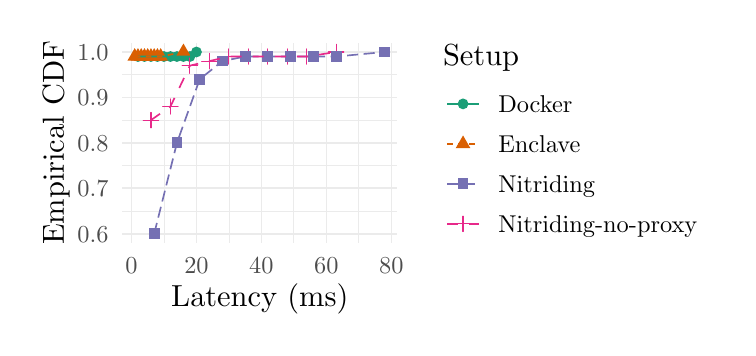
\begin{tikzpicture}[x=1pt,y=1pt]
\definecolor{fillColor}{RGB}{255,255,255}
\path[use as bounding box,fill=fillColor,fill opacity=0.00] (0,0) rectangle (252.94,108.41);
\begin{scope}
\path[clip] ( 34.16, 30.69) rectangle (133.59,102.90);
\definecolor{drawColor}{gray}{0.92}

\path[draw=drawColor,line width= 0.3pt,line join=round] ( 34.16, 42.18) --
	(133.59, 42.18);

\path[draw=drawColor,line width= 0.3pt,line join=round] ( 34.16, 58.59) --
	(133.59, 58.59);

\path[draw=drawColor,line width= 0.3pt,line join=round] ( 34.16, 75.00) --
	(133.59, 75.00);

\path[draw=drawColor,line width= 0.3pt,line join=round] ( 34.16, 91.42) --
	(133.59, 91.42);

\path[draw=drawColor,line width= 0.3pt,line join=round] ( 49.24, 30.69) --
	( 49.24,102.90);

\path[draw=drawColor,line width= 0.3pt,line join=round] ( 72.72, 30.69) --
	( 72.72,102.90);

\path[draw=drawColor,line width= 0.3pt,line join=round] ( 96.20, 30.69) --
	( 96.20,102.90);

\path[draw=drawColor,line width= 0.3pt,line join=round] (119.68, 30.69) --
	(119.68,102.90);

\path[draw=drawColor,line width= 0.6pt,line join=round] ( 34.16, 33.97) --
	(133.59, 33.97);

\path[draw=drawColor,line width= 0.6pt,line join=round] ( 34.16, 50.38) --
	(133.59, 50.38);

\path[draw=drawColor,line width= 0.6pt,line join=round] ( 34.16, 66.80) --
	(133.59, 66.80);

\path[draw=drawColor,line width= 0.6pt,line join=round] ( 34.16, 83.21) --
	(133.59, 83.21);

\path[draw=drawColor,line width= 0.6pt,line join=round] ( 34.16, 99.62) --
	(133.59, 99.62);

\path[draw=drawColor,line width= 0.6pt,line join=round] ( 37.50, 30.69) --
	( 37.50,102.90);

\path[draw=drawColor,line width= 0.6pt,line join=round] ( 60.98, 30.69) --
	( 60.98,102.90);

\path[draw=drawColor,line width= 0.6pt,line join=round] ( 84.46, 30.69) --
	( 84.46,102.90);

\path[draw=drawColor,line width= 0.6pt,line join=round] (107.94, 30.69) --
	(107.94,102.90);

\path[draw=drawColor,line width= 0.6pt,line join=round] (131.42, 30.69) --
	(131.42,102.90);
\definecolor{fillColor}{RGB}{27,158,119}

\path[fill=fillColor] ( 39.85, 97.98) circle (  1.96);

\path[fill=fillColor] ( 42.20, 97.98) circle (  1.96);

\path[fill=fillColor] ( 44.55, 97.98) circle (  1.96);

\path[fill=fillColor] ( 46.89, 97.98) circle (  1.96);

\path[fill=fillColor] ( 49.24, 97.98) circle (  1.96);

\path[fill=fillColor] ( 51.59, 97.98) circle (  1.96);

\path[fill=fillColor] ( 53.94, 97.98) circle (  1.96);

\path[fill=fillColor] ( 56.29, 97.98) circle (  1.96);

\path[fill=fillColor] ( 58.63, 97.98) circle (  1.96);

\path[fill=fillColor] ( 60.98, 99.62) circle (  1.96);
\definecolor{fillColor}{RGB}{217,95,2}

\path[fill=fillColor] ( 38.68,101.03) --
	( 41.32, 96.46) --
	( 36.03, 96.46) --
	cycle;

\path[fill=fillColor] ( 39.85,101.03) --
	( 42.49, 96.46) --
	( 37.21, 96.46) --
	cycle;

\path[fill=fillColor] ( 41.02,101.03) --
	( 43.67, 96.46) --
	( 38.38, 96.46) --
	cycle;

\path[fill=fillColor] ( 42.20,101.03) --
	( 44.84, 96.46) --
	( 39.56, 96.46) --
	cycle;

\path[fill=fillColor] ( 43.37,101.03) --
	( 46.01, 96.46) --
	( 40.73, 96.46) --
	cycle;

\path[fill=fillColor] ( 44.55,101.03) --
	( 47.19, 96.46) --
	( 41.90, 96.46) --
	cycle;

\path[fill=fillColor] ( 45.72,101.03) --
	( 48.36, 96.46) --
	( 43.08, 96.46) --
	cycle;

\path[fill=fillColor] ( 46.89,101.03) --
	( 49.54, 96.46) --
	( 44.25, 96.46) --
	cycle;

\path[fill=fillColor] ( 48.07,101.03) --
	( 50.71, 96.46) --
	( 45.43, 96.46) --
	cycle;

\path[fill=fillColor] ( 56.29,102.67) --
	( 58.93, 98.10) --
	( 53.64, 98.10) --
	cycle;
\definecolor{drawColor}{RGB}{231,41,138}

\path[draw=drawColor,line width= 0.4pt,line join=round,line cap=round] ( 41.77, 75.00) -- ( 47.32, 75.00);

\path[draw=drawColor,line width= 0.4pt,line join=round,line cap=round] ( 44.55, 72.23) -- ( 44.55, 77.78);

\path[draw=drawColor,line width= 0.4pt,line join=round,line cap=round] ( 48.81, 79.93) -- ( 54.36, 79.93);

\path[draw=drawColor,line width= 0.4pt,line join=round,line cap=round] ( 51.59, 77.15) -- ( 51.59, 82.70);

\path[draw=drawColor,line width= 0.4pt,line join=round,line cap=round] ( 55.86, 94.70) -- ( 61.41, 94.70);

\path[draw=drawColor,line width= 0.4pt,line join=round,line cap=round] ( 58.63, 91.92) -- ( 58.63, 97.47);

\path[draw=drawColor,line width= 0.4pt,line join=round,line cap=round] ( 62.90, 96.34) -- ( 68.45, 96.34);

\path[draw=drawColor,line width= 0.4pt,line join=round,line cap=round] ( 65.68, 93.56) -- ( 65.68, 99.11);

\path[draw=drawColor,line width= 0.4pt,line join=round,line cap=round] ( 69.95, 97.98) -- ( 75.50, 97.98);

\path[draw=drawColor,line width= 0.4pt,line join=round,line cap=round] ( 72.72, 95.21) -- ( 72.72,100.76);

\path[draw=drawColor,line width= 0.4pt,line join=round,line cap=round] ( 76.99, 97.98) -- ( 82.54, 97.98);

\path[draw=drawColor,line width= 0.4pt,line join=round,line cap=round] ( 79.77, 95.21) -- ( 79.77,100.76);

\path[draw=drawColor,line width= 0.4pt,line join=round,line cap=round] ( 84.03, 97.98) -- ( 89.58, 97.98);

\path[draw=drawColor,line width= 0.4pt,line join=round,line cap=round] ( 86.81, 95.21) -- ( 86.81,100.76);

\path[draw=drawColor,line width= 0.4pt,line join=round,line cap=round] ( 91.08, 97.98) -- ( 96.63, 97.98);

\path[draw=drawColor,line width= 0.4pt,line join=round,line cap=round] ( 93.85, 95.21) -- ( 93.85,100.76);

\path[draw=drawColor,line width= 0.4pt,line join=round,line cap=round] ( 98.12, 97.98) -- (103.67, 97.98);

\path[draw=drawColor,line width= 0.4pt,line join=round,line cap=round] (100.90, 95.21) -- (100.90,100.76);

\path[draw=drawColor,line width= 0.4pt,line join=round,line cap=round] (108.69, 99.62) -- (114.24, 99.62);

\path[draw=drawColor,line width= 0.4pt,line join=round,line cap=round] (111.46, 96.85) -- (111.46,102.40);
\definecolor{fillColor}{RGB}{117,112,179}

\path[fill=fillColor] ( 43.76, 32.01) --
	( 47.68, 32.01) --
	( 47.68, 35.93) --
	( 43.76, 35.93) --
	cycle;

\path[fill=fillColor] ( 51.98, 64.83) --
	( 55.90, 64.83) --
	( 55.90, 68.76) --
	( 51.98, 68.76) --
	cycle;

\path[fill=fillColor] ( 60.19, 87.81) --
	( 64.12, 87.81) --
	( 64.12, 91.74) --
	( 60.19, 91.74) --
	cycle;

\path[fill=fillColor] ( 68.41, 94.38) --
	( 72.34, 94.38) --
	( 72.34, 98.30) --
	( 68.41, 98.30) --
	cycle;

\path[fill=fillColor] ( 76.63, 96.02) --
	( 80.55, 96.02) --
	( 80.55, 99.94) --
	( 76.63, 99.94) --
	cycle;

\path[fill=fillColor] ( 84.85, 96.02) --
	( 88.77, 96.02) --
	( 88.77, 99.94) --
	( 84.85, 99.94) --
	cycle;

\path[fill=fillColor] ( 93.07, 96.02) --
	( 96.99, 96.02) --
	( 96.99, 99.94) --
	( 93.07, 99.94) --
	cycle;

\path[fill=fillColor] (101.28, 96.02) --
	(105.21, 96.02) --
	(105.21, 99.94) --
	(101.28, 99.94) --
	cycle;

\path[fill=fillColor] (109.50, 96.02) --
	(113.43, 96.02) --
	(113.43, 99.94) --
	(109.50, 99.94) --
	cycle;

\path[fill=fillColor] (127.11, 97.66) --
	(131.03, 97.66) --
	(131.03,101.58) --
	(127.11,101.58) --
	cycle;
\definecolor{drawColor}{RGB}{27,158,119}

\path[draw=drawColor,line width= 0.6pt,line join=round] ( 39.85, 97.98) --
	( 42.20, 97.98) --
	( 44.55, 97.98) --
	( 46.89, 97.98) --
	( 49.24, 97.98) --
	( 51.59, 97.98) --
	( 53.94, 97.98) --
	( 56.29, 97.98) --
	( 58.63, 97.98) --
	( 60.98, 99.62);
\definecolor{drawColor}{RGB}{217,95,2}

\path[draw=drawColor,line width= 0.6pt,dash pattern=on 2pt off 2pt ,line join=round] ( 38.68, 97.98) --
	( 39.85, 97.98) --
	( 41.02, 97.98) --
	( 42.20, 97.98) --
	( 43.37, 97.98) --
	( 44.55, 97.98) --
	( 45.72, 97.98) --
	( 46.89, 97.98) --
	( 48.07, 97.98) --
	( 56.29, 99.62);
\definecolor{drawColor}{RGB}{117,112,179}

\path[draw=drawColor,line width= 0.6pt,dash pattern=on 4pt off 2pt ,line join=round] ( 45.72, 33.97) --
	( 53.94, 66.80) --
	( 62.16, 89.77) --
	( 70.37, 96.34) --
	( 78.59, 97.98) --
	( 86.81, 97.98) --
	( 95.03, 97.98) --
	(103.25, 97.98) --
	(111.46, 97.98) --
	(129.07, 99.62);
\definecolor{drawColor}{RGB}{231,41,138}

\path[draw=drawColor,line width= 0.6pt,dash pattern=on 4pt off 4pt ,line join=round] ( 44.55, 75.00) --
	( 51.59, 79.93) --
	( 58.63, 94.70) --
	( 65.68, 96.34) --
	( 72.72, 97.98) --
	( 79.77, 97.98) --
	( 86.81, 97.98) --
	( 93.85, 97.98) --
	(100.90, 97.98) --
	(111.46, 99.62);
\end{scope}
\begin{scope}
\path[clip] (  0.00,  0.00) rectangle (252.94,108.41);
\definecolor{drawColor}{gray}{0.30}

\node[text=drawColor,anchor=base east,inner sep=0pt, outer sep=0pt, scale=  0.88] at ( 29.21, 30.94) {0.6};

\node[text=drawColor,anchor=base east,inner sep=0pt, outer sep=0pt, scale=  0.88] at ( 29.21, 47.35) {0.7};

\node[text=drawColor,anchor=base east,inner sep=0pt, outer sep=0pt, scale=  0.88] at ( 29.21, 63.77) {0.8};

\node[text=drawColor,anchor=base east,inner sep=0pt, outer sep=0pt, scale=  0.88] at ( 29.21, 80.18) {0.9};

\node[text=drawColor,anchor=base east,inner sep=0pt, outer sep=0pt, scale=  0.88] at ( 29.21, 96.59) {1.0};
\end{scope}
\begin{scope}
\path[clip] (  0.00,  0.00) rectangle (252.94,108.41);
\definecolor{drawColor}{gray}{0.30}

\node[text=drawColor,anchor=base,inner sep=0pt, outer sep=0pt, scale=  0.88] at ( 37.50, 19.68) {0};

\node[text=drawColor,anchor=base,inner sep=0pt, outer sep=0pt, scale=  0.88] at ( 60.98, 19.68) {20};

\node[text=drawColor,anchor=base,inner sep=0pt, outer sep=0pt, scale=  0.88] at ( 84.46, 19.68) {40};

\node[text=drawColor,anchor=base,inner sep=0pt, outer sep=0pt, scale=  0.88] at (107.94, 19.68) {60};

\node[text=drawColor,anchor=base,inner sep=0pt, outer sep=0pt, scale=  0.88] at (131.42, 19.68) {80};
\end{scope}
\begin{scope}
\path[clip] (  0.00,  0.00) rectangle (252.94,108.41);
\definecolor{drawColor}{RGB}{0,0,0}

\node[text=drawColor,anchor=base,inner sep=0pt, outer sep=0pt, scale=  1.10] at ( 83.87,  7.64) {Latency (ms)};
\end{scope}
\begin{scope}
\path[clip] (  0.00,  0.00) rectangle (252.94,108.41);
\definecolor{drawColor}{RGB}{0,0,0}

\node[text=drawColor,rotate= 90.00,anchor=base,inner sep=0pt, outer sep=0pt, scale=  1.10] at ( 13.08, 66.80) {Empirical CDF};
\end{scope}
\begin{scope}
\path[clip] (  0.00,  0.00) rectangle (252.94,108.41);
\definecolor{drawColor}{RGB}{0,0,0}

\node[text=drawColor,anchor=base west,inner sep=0pt, outer sep=0pt, scale=  1.10] at (150.09, 94.67) {Setup};
\end{scope}
\begin{scope}
\path[clip] (  0.00,  0.00) rectangle (252.94,108.41);
\definecolor{fillColor}{RGB}{27,158,119}

\path[fill=fillColor] (157.32, 80.87) circle (  1.96);
\end{scope}
\begin{scope}
\path[clip] (  0.00,  0.00) rectangle (252.94,108.41);
\definecolor{drawColor}{RGB}{27,158,119}

\path[draw=drawColor,line width= 0.6pt,line join=round] (151.54, 80.87) -- (163.10, 80.87);
\end{scope}
\begin{scope}
\path[clip] (  0.00,  0.00) rectangle (252.94,108.41);
\definecolor{fillColor}{RGB}{217,95,2}

\path[fill=fillColor] (157.32, 69.47) --
	(159.96, 64.89) --
	(154.68, 64.89) --
	cycle;
\end{scope}
\begin{scope}
\path[clip] (  0.00,  0.00) rectangle (252.94,108.41);
\definecolor{drawColor}{RGB}{217,95,2}

\path[draw=drawColor,line width= 0.6pt,dash pattern=on 2pt off 2pt ,line join=round] (151.54, 66.42) -- (163.10, 66.42);
\end{scope}
\begin{scope}
\path[clip] (  0.00,  0.00) rectangle (252.94,108.41);
\definecolor{fillColor}{RGB}{117,112,179}

\path[fill=fillColor] (155.36, 50.00) --
	(159.28, 50.00) --
	(159.28, 53.92) --
	(155.36, 53.92) --
	cycle;
\end{scope}
\begin{scope}
\path[clip] (  0.00,  0.00) rectangle (252.94,108.41);
\definecolor{drawColor}{RGB}{117,112,179}

\path[draw=drawColor,line width= 0.6pt,dash pattern=on 4pt off 2pt ,line join=round] (151.54, 51.96) -- (163.10, 51.96);
\end{scope}
\begin{scope}
\path[clip] (  0.00,  0.00) rectangle (252.94,108.41);
\definecolor{drawColor}{RGB}{231,41,138}

\path[draw=drawColor,line width= 0.4pt,line join=round,line cap=round] (154.54, 37.51) -- (160.09, 37.51);

\path[draw=drawColor,line width= 0.4pt,line join=round,line cap=round] (157.32, 34.73) -- (157.32, 40.28);
\end{scope}
\begin{scope}
\path[clip] (  0.00,  0.00) rectangle (252.94,108.41);
\definecolor{drawColor}{RGB}{231,41,138}

\path[draw=drawColor,line width= 0.6pt,dash pattern=on 4pt off 4pt ,line join=round] (151.54, 37.51) -- (163.10, 37.51);
\end{scope}
\begin{scope}
\path[clip] (  0.00,  0.00) rectangle (252.94,108.41);
\definecolor{drawColor}{RGB}{0,0,0}

\node[text=drawColor,anchor=base west,inner sep=0pt, outer sep=0pt, scale=  0.88] at (170.05, 77.84) {Docker};
\end{scope}
\begin{scope}
\path[clip] (  0.00,  0.00) rectangle (252.94,108.41);
\definecolor{drawColor}{RGB}{0,0,0}

\node[text=drawColor,anchor=base west,inner sep=0pt, outer sep=0pt, scale=  0.88] at (170.05, 63.38) {Enclave};
\end{scope}
\begin{scope}
\path[clip] (  0.00,  0.00) rectangle (252.94,108.41);
\definecolor{drawColor}{RGB}{0,0,0}

\node[text=drawColor,anchor=base west,inner sep=0pt, outer sep=0pt, scale=  0.88] at (170.05, 48.93) {Nitriding};
\end{scope}
\begin{scope}
\path[clip] (  0.00,  0.00) rectangle (252.94,108.41);
\definecolor{drawColor}{RGB}{0,0,0}

\node[text=drawColor,anchor=base west,inner sep=0pt, outer sep=0pt, scale=  0.88] at (170.05, 34.48) {Nitriding-no-proxy};
\end{scope}
\end{tikzpicture}
